\newcommand{\pitcharray}{%
  \dflat D, \dflat A, \dflat E, \dflat B, \flat F,
  \flat C, \flat G, \flat D, \flat A, \flat E,
  \flat B, F, C, G, D, A, E, B,
  \sharp F, \sharp C, \sharp G, \sharp D, \sharp A, \sharp E, \sharp B}
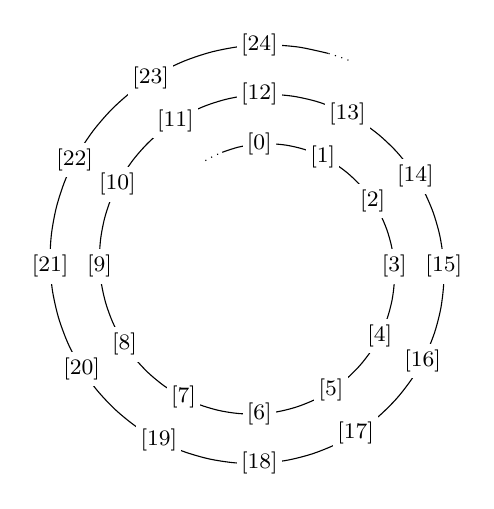
\begin{tikzpicture}[xscale=-1]
  \def\xA{1.4}
  \def\xB{.1}
  \draw[dotted,domain=.35*pi:.4*pi,smooth,samples=100,variable=\t]
  plot ({(\xA+\xB*\t)*cos(\t r)},{(\xA+\xB*\t)*sin(\t r)});
  \draw[domain=.4*pi:4.6*pi,smooth,samples=100,variable=\t]
  plot ({(\xA+\xB*\t)*cos(\t r)},{(\xA+\xB*\t)*sin(\t r)});
  \draw[dotted,domain=4.6*pi:4.63*pi,smooth,samples=100,variable=\t]
  plot ({(\xA+\xB*\t)*cos(\t r)},{(\xA+\xB*\t)*sin(\t r)});
  \foreach \i in {0,...,24}{
    \node[fill=white,inner sep=1.5px]
    at ({(\xA+\xB*(\i+3)*pi/6)*cos((\i+3)*pi/6 r)},
    {(\xA+\xB*(\i+3)*pi/6)*sin((\i+3)*pi/6 r)})
    {\footnotesize \pitch[\i]$\strut$};
  };
\end{tikzpicture}
